% $Header: /u/gcmpack/manual/s_examples/global_oce_latlon/climatalogical_ogcm.tex,v 1.25 2015/11/25 10:57:41 mlosch Exp $
% $Name:  $

\section[Global Ocean MITgcm Example]{Global Ocean Simulation at $4^\circ$ Resolution}
%\label{www:tutorials}
\label{sec:eg-global}
\begin{rawhtml}
<!-- CMIREDIR:eg-global: -->
\end{rawhtml}
\begin{center}
(in directory: {\it verification/tutorial\_global\_oce\_latlon/})
\end{center}

\bodytext{bgcolor="#FFFFFFFF"}

\noindent {\bf WARNING: the description of this experiment is not complete.
 In particular, many parameters are not yet described.}\\

%\begin{center}
%{\Large \bf Using MITgcm to Simulate Global Climatological Ocean Circulation
%At Four Degree Resolution with Asynchronous Time Stepping}
%
%\vspace*{4mm}
%
%\vspace*{3mm}
%{\large May 2001}
%\end{center}

This example experiment demonstrates using the MITgcm to simulate the
planetary ocean circulation. The simulation is configured with
realistic geography and bathymetry on a $4^{\circ} \times 4^{\circ}$
spherical polar grid. The files for this experiment are in the
verification directory under tutorial\_global\_oce\_latlon. Fifteen
levels are used in the vertical, ranging in thickness from $50\,{\rm
  m}$ at the surface to $690\,{\rm m}$ at depth, giving a maximum
model depth of $5200\,{\rm m}$.
Different time-steps are used to accelerate the convergence to
equilibrium \cite[]{bryan:84} so that, at this resolution,
the configuration can be integrated forward for thousands of years
on a single processor desktop computer.
\\
\subsection{Overview}
%\label{www:tutorials}

The model is forced with climatological wind stress data from
\citet{trenberth90} and NCEP surface flux data from
\citet{kalnay96}. Climatological data \citep{Levitus94} is
used to initialize the model hydrography. \citeauthor{Levitus94} seasonal
climatology data is also used throughout the calculation to provide
additional air-sea fluxes.  These fluxes are combined with the NCEP
climatological estimates of surface heat flux, resulting in a mixed
boundary condition of the style described in \citet{Haney}.
Altogether, this yields the following forcing applied in the model
surface layer.

\begin{eqnarray}
\label{eq:eg-global-global_forcing}
\label{eq:eg-global-global_forcing_fu}
{\cal F}_{u} & = & \frac{\tau_{x}}{\rho_{0} \Delta z_{s}}
\\
\label{eq:eg-global-global_forcing_fv}
{\cal F}_{v} & = & \frac{\tau_{y}}{\rho_{0} \Delta z_{s}}
\\
\label{eq:eg-global-global_forcing_ft}
{\cal F}_{\theta} & = & - \lambda_{\theta} ( \theta - \theta^{\ast} )
 - \frac{1}{C_{p} \rho_{0} \Delta z_{s}}{\cal Q}
\\
\label{eq:eg-global-global_forcing_fs}
{\cal F}_{s} & = & - \lambda_{s} ( S - S^{\ast} )
 + \frac{S_{0}}{\Delta z_{s}}({\cal E} - {\cal P} - {\cal R})
\end{eqnarray}

\noindent where ${\cal F}_{u}$, ${\cal F}_{v}$, ${\cal F}_{\theta}$,
${\cal F}_{s}$ are the forcing terms in the zonal and meridional
momentum and in the potential temperature and salinity
equations respectively.
The term $\Delta z_{s}$ represents the top ocean layer thickness in
meters.
It is used in conjunction with a reference density, $\rho_{0}$
(here set to $999.8\,{\rm kg\,m^{-3}}$), a
reference salinity, $S_{0}$ (here set to 35~ppt),
and a specific heat capacity, $C_{p}$ (here set to
$4000~{\rm J}~^{\circ}{\rm C}^{-1}~{\rm kg}^{-1}$), to convert
input dataset values into time tendencies of
potential temperature (with units of $^{\circ}{\rm C}~{\rm s}^{-1}$),
salinity (with units ${\rm ppt}~s^{-1}$) and
velocity (with units ${\rm m}~{\rm s}^{-2}$).
The externally supplied forcing fields used in this
experiment are $\tau_{x}$, $\tau_{y}$, $\theta^{\ast}$, $S^{\ast}$,
$\cal{Q}$ and $\cal{E}-\cal{P}-\cal{R}$. The wind stress fields ($\tau_x$, $\tau_y$)
have units of ${\rm N}~{\rm m}^{-2}$. The temperature forcing fields
($\theta^{\ast}$ and $Q$) have units of $^{\circ}{\rm C}$ and ${\rm W}~{\rm m}^{-2}$
respectively. The salinity forcing fields ($S^{\ast}$ and
$\cal{E}-\cal{P}-\cal{R}$) have units of ${\rm ppt}$ and ${\rm m}~{\rm s}^{-1}$
respectively. The source files and procedures for ingesting this data into the
simulation are described in the experiment configuration discussion in section
\ref{sec:eg-global-clim_ocn_examp_exp_config}.


\subsection{Discrete Numerical Configuration}
%\label{www:tutorials}


The model is configured in hydrostatic form.  The domain is
discretised with a uniform grid spacing in latitude and longitude on
the sphere $\Delta \phi=\Delta \lambda=4^{\circ}$, so that there are
ninety grid cells in the zonal and forty in the meridional
direction. The internal model coordinate variables $x$ and $y$ are
initialized according to
\begin{eqnarray}
x=r\cos(\phi),~\Delta x & = &r\cos(\Delta \phi) \\
y=r\lambda,~\Delta y &= &r\Delta \lambda
\end{eqnarray}

Arctic polar regions are not
included in this experiment. Meridionally the model extends from
$80^{\circ}{\rm S}$ to $80^{\circ}{\rm N}$.
Vertically the model is configured with fifteen layers with the
following thicknesses:
$\Delta z_{1} = 50\,{\rm m},$\\
$\Delta z_{2} = 70\,{\rm m},\,
 \Delta z_{3} = 100\,{\rm m},\,
 \Delta z_{4} = 140\,{\rm m},\,
 \Delta z_{5} = 190\,{\rm m},\,
 \Delta z_{6} = 240\,{\rm m},\,
 \Delta z_{7} = 290\,{\rm m},\,
 \Delta z_{8} = 340\,{\rm m},$\\
$\Delta z_{9} = 390\,{\rm m},\,
 \Delta z_{10}= 440\,{\rm m},\,
 \Delta z_{11}= 490\,{\rm m},\,
 \Delta z_{12}= 540\,{\rm m},\,
 \Delta z_{13}= 590\,{\rm m},\,
 \Delta z_{14}= 640\,{\rm m},\,
 \Delta z_{15}= 690\,{\rm m}$\\
(here the numeric subscript indicates the model level index number, ${\tt k}$) to
give a total depth, $H$, of $-5200{\rm m}$.
The implicit free surface form of the pressure equation described in
\citet{marshall:97a} is employed. A Laplacian operator, $\nabla^2$, provides viscous
dissipation. Thermal and haline diffusion is also represented by a Laplacian operator.

Wind-stress forcing is added to the momentum equations in (\ref{eq:eg-global-model_equations})
for both the zonal flow, $u$ and the meridional flow $v$, according to equations
(\ref{eq:eg-global-global_forcing_fu}) and (\ref{eq:eg-global-global_forcing_fv}).
Thermodynamic forcing inputs are added to the equations
in (\ref{eq:eg-global-model_equations}) for
potential temperature, $\theta$, and salinity, $S$, according to equations
(\ref{eq:eg-global-global_forcing_ft}) and (\ref{eq:eg-global-global_forcing_fs}).
This produces a set of equations solved in this configuration as follows:

\begin{eqnarray}
\label{eq:eg-global-model_equations}
\frac{Du}{Dt} - fv +
  \frac{1}{\rho}\frac{\partial p^{'}}{\partial x} -
  \nabla_{h}\cdot A_{h}\nabla_{h}u -
  \frac{\partial}{\partial z}A_{z}\frac{\partial u}{\partial z}
 & = &
\begin{cases}
{\cal F}_u & \text{(surface)} \\
0 & \text{(interior)}
\end{cases}
\\
\frac{Dv}{Dt} + fu +
  \frac{1}{\rho}\frac{\partial p^{'}}{\partial y} -
  \nabla_{h}\cdot A_{h}\nabla_{h}v -
  \frac{\partial}{\partial z}A_{z}\frac{\partial v}{\partial z}
& = &
\begin{cases}
{\cal F}_v & \text{(surface)} \\
0 & \text{(interior)}
\end{cases}
\\
\frac{\partial \eta}{\partial t} + \nabla_{h}\cdot \vec{u}
&=&
0
\\
\frac{D\theta}{Dt} -
 \nabla_{h}\cdot K_{h}\nabla_{h}\theta
 - \frac{\partial}{\partial z}\Gamma(K_{z})\frac{\partial\theta}{\partial z}
& = &
\begin{cases}
{\cal F}_\theta & \text{(surface)} \\
0 & \text{(interior)}
\end{cases}
\\
\frac{D s}{Dt} -
 \nabla_{h}\cdot K_{h}\nabla_{h}s
 - \frac{\partial}{\partial z}\Gamma(K_{z})\frac{\partial s}{\partial z}
& = &
\begin{cases}
{\cal F}_s & \text{(surface)} \\
0 & \text{(interior)}
\end{cases}
\\
g\rho_{0} \eta + \int^{0}_{-z}\rho^{'} dz & = & p^{'}
\end{eqnarray}

\noindent where $u=\frac{Dx}{Dt}=r \cos(\phi)\frac{D \lambda}{Dt}$ and
$v=\frac{Dy}{Dt}=r \frac{D \phi}{Dt}$
are the zonal and meridional components of the
flow vector, $\vec{u}$, on the sphere. As described in
MITgcm Numerical Solution Procedure \ref{chap:discretization}, the time
evolution of potential temperature, $\theta$, equation is solved prognostically.
The total pressure, $p$, is diagnosed by summing pressure due to surface
elevation $\eta$ and the hydrostatic pressure.
\\

\subsubsection{Numerical Stability Criteria}
%\label{www:tutorials}

The Laplacian dissipation coefficient, $A_{h}$, is set to $5 \times 10^5 m s^{-1}$.
This value is chosen to yield a Munk layer width \citep{adcroft:95},
\begin{eqnarray}
\label{eq:eg-global-munk_layer}
&& M_{w} = \pi ( \frac { A_{h} }{ \beta } )^{\frac{1}{3}}
\end{eqnarray}

\noindent  of $\approx 600$km. This is greater than the model
resolution in low-latitudes, $\Delta x \approx 400{\rm km}$, ensuring that the frictional
boundary layer is adequately resolved.
\\

\noindent The model is stepped forward with a time step $\Delta
t_{\theta}=24~{\rm hours}$ for thermodynamic variables and $\Delta
t_{v}=30~{\rm minutes}$ for momentum terms. With this time step,
the stability parameter to the horizontal Laplacian friction
\citep{adcroft:95}
\begin{eqnarray}
\label{eq:eg-global-laplacian_stability}
&& S_{l} = 4 \frac{A_{h} \Delta t_{v}}{{\Delta x}^2}
\end{eqnarray}

\noindent evaluates to 0.6 at a latitude of $\phi=80^{\circ}$, which
is above the 0.3 upper limit for stability, but the zonal grid spacing
$\Delta x$ is smallest at $\phi=80^{\circ}$ where $\Delta
x=r\cos(\phi)\Delta \phi\approx 77{\rm km}$ and the stability
criterion is already met 1 grid cell equatorwards (at $\phi=76^{\circ}$).


\noindent The vertical dissipation coefficient, $A_{z}$, is set to
$1\times10^{-3} {\rm m}^2{\rm s}^{-1}$. The associated stability limit
\begin{eqnarray}
\label{eq:eg-global-laplacian_stability_z}
&& S_{l} = 4 \frac{A_{z} \Delta t_{v}}{{\Delta z}^2}
\end{eqnarray}

\noindent evaluates to $0.0029$ for the smallest model
level spacing ($\Delta z_{1}=50{\rm m}$) which is well below
the upper stability limit.
\\

% The values of the horizontal ($K_{h}$) and vertical ($K_{z}$) diffusion coefficients
% for both temperature and salinity are set to $1 \times 10^{3}~{\rm m}^{2}{\rm s}^{-1}$
% and $3 \times 10^{-5}~{\rm m}^{2}{\rm s}^{-1}$ respectively. The stability limit
% related to $K_{h}$ will be at $\phi=80^{\circ}$ where $\Delta x \approx 77 {\rm km}$.
% Here the stability parameter
% \begin{eqnarray}
% \label{eq:eg-global-laplacian_stability_xtheta}
% S_{l} = \frac{4 K_{h} \Delta t_{\theta}}{{\Delta x}^2}
% \end{eqnarray}
% evaluates to $0.07$, well below the stability limit of $S_{l} \approx 0.5$. The
% stability parameter related to $K_{z}$
% \begin{eqnarray}
% \label{eq:eg-global-laplacian_stability_ztheta}
% S_{l} = \frac{4 K_{z} \Delta t_{\theta}}{{\Delta z}^2}
% \end{eqnarray}
% evaluates to $0.005$ for $\min(\Delta z)=50{\rm m}$, well below the stability limit
% of $S_{l} \approx 0.5$.
% \\

\noindent The numerical stability for inertial oscillations
\citep{adcroft:95}

\begin{eqnarray}
\label{eq:eg-global-inertial_stability}
&& S_{i} = f^{2} {\Delta t_v}^2
\end{eqnarray}

\noindent evaluates to $0.07$ for
$f=2\omega\sin(80^{\circ})=1.43\times10^{-4}~{\rm s}^{-1}$, which is
below the $S_{i} < 1$ upper limit for stability.
\\

\noindent The advective CFL \citep{adcroft:95} for a extreme maximum
horizontal flow
speed of $ | \vec{u} | = 2 ms^{-1}$

\begin{eqnarray}
\label{eq:eg-global-cfl_stability}
&& S_{a} = \frac{| \vec{u} | \Delta t_{v}}{ \Delta x}
\end{eqnarray}

\noindent evaluates to $5 \times 10^{-2}$. This is well below the stability
limit of 0.5.
\\

\noindent The stability parameter for internal gravity waves propagating
 with a maximum speed of $c_{g}=10~{\rm ms}^{-1}$
\citep{adcroft:95}

\begin{eqnarray}
\label{eq:eg-global-gfl_stability}
&& S_{c} = \frac{c_{g} \Delta t_{v}}{ \Delta x}
\end{eqnarray}

\noindent evaluates to $2.3 \times 10^{-1}$. This is close to the linear
stability limit of 0.5.

\subsection{Experiment Configuration}
%\label{www:tutorials}
\label{sec:eg-global-clim_ocn_examp_exp_config}

The model configuration for this experiment resides under the
directory {\it tutorial\_global\_oce\_latlon/}. The experiment files

\begin{itemize}
\item {\it input/data}
\item {\it input/data.pkg}
\item {\it input/eedata},
\item {\it input/trenberth\_taux.bin},
\item {\it input/trenberth\_tauy.bin},
\item {\it input/lev\_s.bin},
\item {\it input/lev\_t.bin},
\item {\it input/lev\_sss.bin},
\item {\it input/lev\_sst.bin},
\item {\it input/bathymetry.bin},
%\item {\it code/CPP\_EEOPTIONS.h}
%\item {\it code/CPP\_OPTIONS.h},
\item {\it code/SIZE.h}.
\end{itemize}
contain the code customizations and parameter settings for these
experiments. Below we describe the customizations
to these files associated with this experiment.

\subsubsection{Driving Datasets}
%\label{www:tutorials}

%% New figures are included before
%% Relaxation temperature
%\begin{figure}
%\centering
%\includegraphics[]{relax_temperature.eps}
%\caption{Relaxation temperature for January}
%\label{fig:relax_temperature}
%\end{figure}

%% Relaxation salinity
%\begin{figure}
%\centering
%\includegraphics[]{relax_salinity.eps}
%\caption{Relaxation salinity for January}
%\label{fig:relax_salinity}
%\end{figure}

%% tau_x
%\begin{figure}
%\centering
%\includegraphics[]{tau_x.eps}
%\caption{zonal wind stress for January}
%\label{fig:tau_x}
%\end{figure}

%% tau_y
%\begin{figure}
%\centering
%\includegraphics[]{tau_y.eps}
%\caption{meridional wind stress for January}
%\label{fig:tau_y}
%\end{figure}

%% Qnet
%\begin{figure}
%\centering
%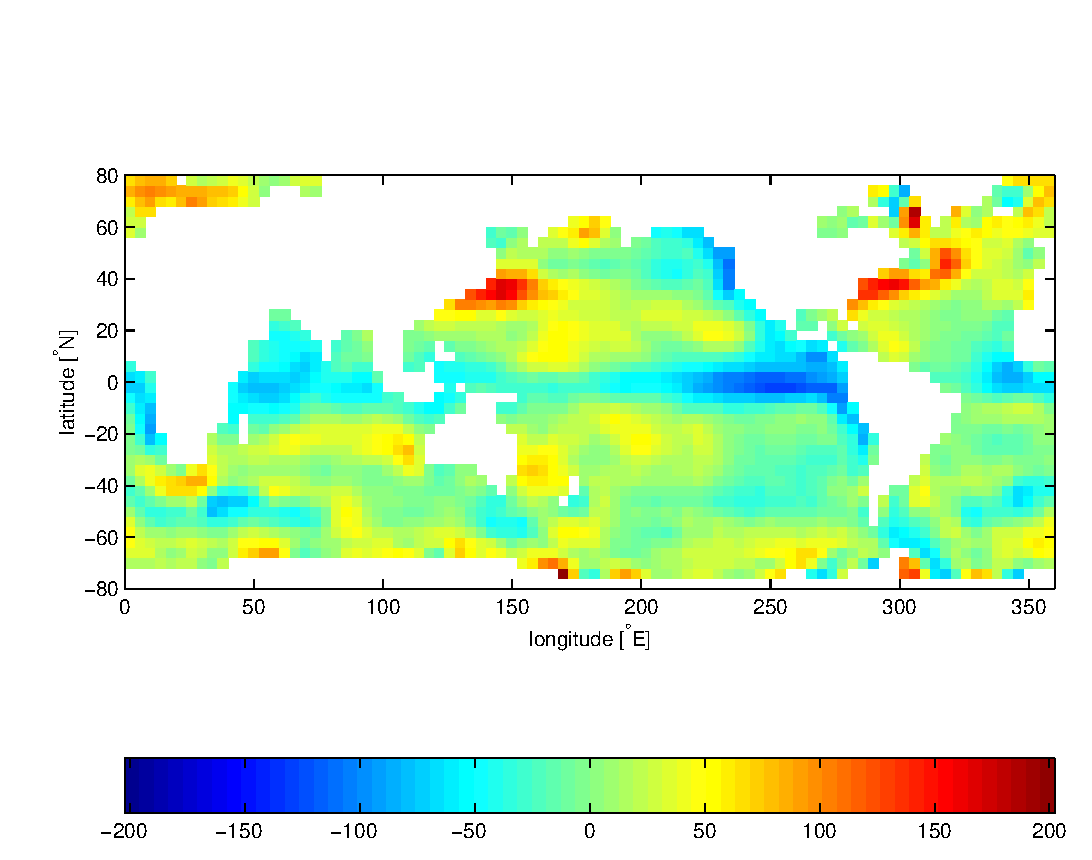
\includegraphics[]{qnet.eps}
%\caption{Heat flux for January}
%\label{fig:qnet}
%\end{figure}

%% EmPmR
%\begin{figure}
%\centering
%\includegraphics[]{empmr.eps}
%\caption{Fresh water flux for January}
%\label{fig:empmr}
%\end{figure}

%% Bathymetry
%\begin{figure}
%\centering
%\includegraphics[]{bathymetry.eps}
%\caption{Bathymetry}
%\label{fig:bathymetry}
%\end{figure}


Figures (\ref{fig:sim_config_tclim_pcoord}-\ref{fig:sim_config_empmr_pcoord})
%(\ref{fig:sim_config_tclim}-\ref{fig:sim_config_empmr})
show the relaxation temperature ($\theta^{\ast}$) and salinity ($S^{\ast}$)
fields, the wind stress components ($\tau_x$ and $\tau_y$), the heat flux ($Q$)
and the net fresh water flux (${\cal E} - {\cal P} - {\cal R}$) used
in equations
(\ref{eq:eg-global-global_forcing_fu}-\ref{eq:eg-global-global_forcing_fs}).
The figures also indicate the lateral extent and coastline used in the
experiment. Figure ({\it --- missing figure --- }) %ref{fig:model_bathymetry})
shows the depth contours of the model domain.

\subsubsection{File {\it input/data}}
%\label{www:tutorials}

\input{s_examples/global_oce_latlon/inp_data}

\subsubsection{File {\it input/data.pkg}}
%\label{www:tutorials}

This file uses standard default values and does not contain
customisations for this experiment.

\subsubsection{File {\it input/eedata}}
%\label{www:tutorials}

This file uses standard default values and does not contain
customisations for this experiment.

\subsubsection{Files{\it input/trenberth\_taux.bin} and {\it
  input/trenberth\_tauy.bin}}
%\label{www:tutorials}

The {\it input/trenberth\_taux.bin} and {\it
  input/trenberth\_tauy.bin} files specify a three-dimensional
($x,y,time$) map of wind stress, $(\tau_{x},\tau_{y})$, values
\citep{trenberth90}. The units used are $Nm^{-2}$.

\subsubsection{File {\it input/bathymetry.bin}}
%\label{www:tutorials}

The {\it input/bathymetry.bin} file specifies a two-dimensional
($x,y$) map of depth values. For this experiment values range
between~$0$ and $-5200\,{\rm m}$, and have been derived from
ETOPO5. The file contains a raw binary stream of data that is
enumerated in the same way as standard MITgcm two-dimensional,
horizontal arrays.

\subsubsection{File {\it code/SIZE.h}}
%\label{www:tutorials}

\input{s_examples/global_oce_latlon/cod_SIZE.h}

%\subsubsection{File {\it code/CPP\_OPTIONS.h}}
%\label{www:tutorials}

%This file uses standard default values and does not contain
%customisations for this experiment.


%\subsubsection{File {\it code/CPP\_EEOPTIONS.h}}
%\label{www:tutorials}

%This file uses standard default values and does not contain
%customisations for this experiment.

\subsubsection{Other Files }
%\label{www:tutorials}

% Other files relevant to this experiment are
% \begin{itemize}
% \item {\it model/src/ini\_cori.F}. This file initializes the model
% coriolis variables {\bf fCorU}.
% \item {\it model/src/ini\_spherical\_polar\_grid.F}
% \item {\it model/src/ini\_parms.F},
% \item {\it input/windx.sin\_y},
% \end{itemize}
% contain the code customisations and parameter settings for this
% experiments. Below we describe the customisations
% to these files associated with this experiment.
